
\documentclass{article}
\usepackage[landscape]{geometry}
\usepackage{url}
\usepackage{multicol}
\usepackage{amsmath}
\usepackage{esint}
\usepackage{amsfonts}
\usepackage{tikz}
\usetikzlibrary{decorations.pathmorphing}
\usepackage{amsmath,amssymb}
\usepackage{pgfplots,caption}
\usepackage{graphicx}

\usepackage{colortbl}
\usepackage{xcolor}
\usepackage{mathtools}
\usepackage{amsmath,amssymb}
\usepackage{enumitem}
\makeatletter

\newcommand*\bigcdot{\mathpalette\bigcdot@{.5}}
\newcommand*\bigcdot@[2]{\mathbin{\vcenter{\hbox{\scalebox{#2}{$\m@th#1\bullet$}}}}}
\makeatother

\title{130 Cheat Sheet}
\usepackage[brazilian]{babel}
\usepackage[utf8]{inputenc}

\advance\topmargin-.8in
\advance\textheight3in
\advance\textwidth3in
\advance\oddsidemargin-1.5in
\advance\evensidemargin-1.5in
\parindent0pt
\parskip2pt
\newcommand{\hr}{\centerline{\rule{3.5in}{1pt}}}
%\colorbox[HTML]{e4e4e4}{\makebox[\textwidth-2\fboxsep][l]{texto}
\begin{document}
	
	\begin{center}{\huge{\textbf{Reinforcement Learning Cheat Sheet}}}\\
	\end{center}
	\begin{multicols*}{3}
		
		\tikzstyle{mybox} = [draw=black, fill=white, very thick,
		rectangle, rounded corners, inner sep=10pt, inner ysep=10pt]
		\tikzstyle{fancytitle} =[fill=black, text=white, font=\bfseries]
		
		%------------ Notation ---------------
		\begin{tikzpicture}
		\node [mybox] (box){%
			\begin{minipage}{0.3\textwidth}
				In general, random variables are upper case and the values of the random variable are lower case. Matrices are bold. \\

				\begin{tabular}{lp{5cm} l}
				Symbol   & Meaning \\
				$t$ & a discrete time\\
				$S_t$ & state at time t \\
				$A_t$ & action at time t \\
				$R_t$ & reward at time t \\
				$\mathcal{S}$ & set of all non-terminal states \\
				$ \mathcal{A}$ & set of all actions \\
				$ \mathcal{R}$ & set of all rewards 
				\end{tabular}

			\end{minipage}
		};
		%------------ Notation Header ---------------------
		\node[fancytitle, right=10pt] at (box.north west) {Notation};
		\end{tikzpicture}
		
		%------------ MDP ---------------
		\begin{tikzpicture}
		\node [mybox] (box){%
			\begin{minipage}{0.3\textwidth}
			 
			\begin{center}
			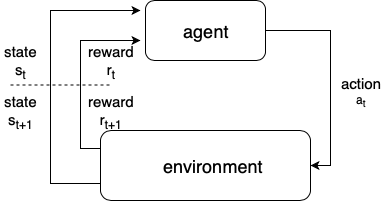
\includegraphics[width=6cm]{../img/env.png}
			\captionof{figure}{Actor-critic relation}
			\label{plot:env}
			\end{center}

			

			
			In a Markov decision process shown in Figure \ref{plot:env}, a game agent interacts with an environment to achieve a certain goal. The interaction happens at every discrete time $ t = 1, 2, 3, ... $. The agent observes certain state of the environment $ S_t \in \mathcal{S} $, selects some action $ A_t \in \mathcal{A} $ and then receives certain reward $ R_{t+1} \in \mathcal{R} $. A policy $\pi$ take
			\end{minipage}
		};
		%------------ MDP Header ---------------------
		\node[fancytitle, right=10pt] at (box.north west) {Problem setup: Markov decision processes};
		\end{tikzpicture}
		
		%------------ AC ---------------
		\begin{tikzpicture}
		\node [mybox] (box){%
			\begin{minipage}{0.3\textwidth}

			\begin{center}
				\begin{tikzpicture}
				\draw (2.0, 2) node[align=left] {Value \\  based \\ methods};
				\draw (4.0, 2) node[align=left] {Actor \\ critic};
				\draw (6.0, 2) node[align=left] {Policy \\  gradient \\ methods};
				\draw (3,2) circle (2.0cm) ;
				\draw (5,2) circle (2.0cm);
				\end{tikzpicture}
				\captionof{figure}{Actor-critic relation}
				\label{plot:ac}
			\end{center}

			Actor-critic  (AC) methods lay between value-based and policy gradient methods as shown in figure \ref{plot:ac}. They both estimate the policy and state-action functions, whereas value-based methods only estimate state-value functions and have an implicit $\epsilon$-greedy policy, and policy gradient methods do not have value function and only estimates the policy.
			\end{minipage}
		};
		%------------ AC Header ---------------------
		\node[fancytitle, right=10pt] at (box.north west) {Actor-critic};
		\end{tikzpicture}
		
		%------------ Variation of Parameters Content ---------------------
		\begin{tikzpicture}
		\node [mybox] (box){%
			\begin{minipage}{0.3\textwidth}
			\begin{align*}
			F(x) &= y'' + y' \\
			y_h &= b_1y_1(x) + b_2y_2(x), y_1 y_2 \text{ are L.I.} \\
			y_p &= u_1(x)y_1(x) + u_2(x)y_2(x) \\
			u_1 &= \int^t -\frac{y_2F(t)dt}{w[y_1,y_2](t)} \\
			u_2 &= \int^t \frac{y_1F(t)dt}{w[y_1,y_2](t)} \\    		
			y &= y_h + y_p
			\end{align*}
			\end{minipage}
		};
		%------------ Variation of Parameters Header ---------------------
		\node[fancytitle, right=10pt] at (box.north west) {Variation of Parameters};
		\end{tikzpicture}
		
		%------------ ODE Content ---------------
		\begin{tikzpicture}
		\node [mybox] (box){%
			\begin{minipage}{0.3\textwidth}
			\small{
				\begin{tabular}{lp{4cm} l}
				\textit{1st Order Linear} & Use integrating factor,
				\\ & $I = e^{\int P(x) dx}$ \\ \hline
				\textit{Separable:} & $ \int P(y) dy/dx = \int Q(x) $ \\ \hline
				\textit{HomogEnEous:} & $ dy/dx = f(x,y) = f(xt,yt) $ \\ &
				sub $ y = xV $ solve, then sub $ V = y/x $ \\ \hline
				\textit{Exact:} & If $ M(x,y) + N(x,y)dy/dx = 0 $ and $ M_y = N_x $ i.e. $ \langle M,N \rangle = \nabla F $ then $ \int_x M + \int_y N = F $ \\ \hline
				\textit{Order Reduction} & Let $ v = dy/dx $ then check other types \\ 
				&\textit{If purely a function of y, }$\frac{dv}{dx} = v\frac{dv}{dy}$\\
				\hline
				\textit{Variation of Parameters:} & When $y''+a_1y'+a_2y = F(x)$ \\
				& $F$ contains $\ln x$, $\sec x$, $\tan x$, $\div$ \\ \hline
				\textit{Bernoulli} & $y' + P(x)y = Q(x)y^n$ \\
				& $\div y^n$ \\
				&$y^{-n}y'+P(x)y^{1-n}=Q(x)$ \textit{Let }$U(x) = y^{1-n}(x)$ \\
				&$\frac{dU}{dx}=(1-n)y^{-n}\frac{dy}{dx}$ \\
				&$\frac{1}{1-n}\frac{du}{dx} + P(x)U(x) = Q(x)$ \textit{solve as a 1st order} \\ \hline
				\textit{Cauchy-Euler} &$x^ny^n + a_1x^{n-1}y^{n-1} + \cdots + a_{n-1}y^{n-2}+a_ny = 0$ \\
				&guess $y = x^r$ \\
				\textit{3 Cases:} \\
				\textit{1) Distinct real roots} &$y = ax^{r_1}+bx^{r_2}$ \\
				\textit{2) Repeated real roots} &$y = Ax^r + y_2$ \\
				&\textit{Guess} $y_2 = x^ru(x)$ \\
				&\textit{Solve for $u(x)$ and choose one ($A=1, C=0$)} \\
				\textit{3) Distinct complex roots} &$y=B_1x^a \cos (b \ln x) + B_2x^a\sin (b \ln x)$
				\end{tabular}}
			\end{minipage}
		};
		%------------ ODE Header ---------------------
		\node[fancytitle, right=10pt] at (box.north west) {ODEs};
		\end{tikzpicture}
		
		%------------ Series Solution Content ---------------
		\begin{tikzpicture}
		\node [mybox] (box){%
			\begin{minipage}{0.3\textwidth}
			$y'' + p(x)y' + q(x)y = 0$ \\
			Useful when $p(x), q(x)$ not constant \\
			Guess $y = \sum_{n=0}^{\infty}a_n(x-x_0)^n$
			\small{
				\begin{tabular}{lp{4cm} l}
				\hline
				$e^x$ & $\sum_{n=0}^{\infty} x^n/{n!}$ \\ \hline
				$\sin x$ & $\sum_{n=0}^{\infty} \frac{(-1)^n}{(2n+1)!}x^{2n+1}$ \\ \hline
				$\cos x$ & $\sum_{n=0}^{\infty} \frac{(-1)^n}{(2n)!}x^{2n}$ \\
				\end{tabular}}
			\end{minipage}
		};
		%------------ Series Solution Header ---------------------
		\node[fancytitle, right=10pt] at (box.north west) {Series Solution};
		\end{tikzpicture}
		
		%------------ Systems of ODE Content ---------------
		\begin{tikzpicture}
		\node [mybox] (box){%
			\begin{minipage}{0.3\textwidth}
			\small{
				\begin{tabular}{lp{4cm} l}
				$\vec{x}' = A\vec{x}$ \\
				\textit{A is diagonalizable} & $\vec{x}(t)=a_{1}e^{\lambda_1 t}\vec{v_1}+\cdots+ a_{n}e^{\lambda_n t}\vec{v_n}$ \\ \hline
				\textit{A is not diagonalizable} & $\vec{x}(t)=a_1e^{\lambda_1 t}\vec{v_1} + a_2e^{\lambda t}(\vec{w} + t\vec{v} )$ \\
				& where $(A - \lambda I)\vec{w} = \vec{v} $\\
				& $\vec{v}$ is an Eigenvector w/ value $\lambda$ \\
				& i.e. $\vec{w}$ is a generalized Eigenvector \\ \hline
				$\vec{x}' = A\vec{x} + \vec{B}$ &Solve $y_h$ \\
				& $\vec{x_1} = e^{\lambda_1t}\vec{v_1}, \vec{x_2} = e^{\lambda_2t}\vec{v_2}$ \\ 			& $\vec{X} = [\vec{x_1},\vec{x_2}]$ \\
				& $\vec{X}\vec{u}'=\vec{B}$ \\
				& $y_p = \vec{X}\vec{u}$ \\
				& $y = y_h + y_p$
				\end{tabular}}
			\end{minipage}
		};
		%------------ Systems of ODE Header ---------------------
		\node[fancytitle, right=10pt] at (box.north west) {Systems};
		\end{tikzpicture}
		
		%------------ Exponentiation Content ---------------
		\begin{tikzpicture}
		\node [mybox] (box){%
			\begin{minipage}{0.3\textwidth}
			\small{
				\begin{tabular}{lp{4cm} l}
				$A^n = SD^nS^{-1}$ \\
				\textit{D is the diagonalization of A}
				\end{tabular}}
			\end{minipage}
		};
		%------------ Spring-Mass Header ---------------------
		\node[fancytitle, right=10pt] at (box.north west) {Matrix Exponentiation};
		\end{tikzpicture}
		\
		%------------ Laplace Transforms Content ---------------
		\begin{tikzpicture}
		\node [mybox] (box){%
			\begin{minipage}{0.3\textwidth}
			$L[f](s) = \int_0^{\infty} e^{-sx}f(x)dx $\\
			
			\small{
				\begin{tabular}{lp{4cm} l}
				$f(t) = t^n, n \geq 0 $ &$F(s) = \frac{n!}{s^{n+1}}, s > 0 $ \\
				$f(t) = e^{at}, a \textit{ constant}$ & $ F(s) = \frac{1}{s-a}, s > a$ \\
				$f(t) = \sin{bt}, b \textit{ constant}$ & $ F(s) = \frac{b}{s^2 + b^2}, s > 0$ \\
				$f(t) = \cos{bt}, b \textit{ constant}$ & $ F(s) = \frac{s}{s^2 + b^2}, s > 0$ \\
				$f(t) = t^{-1/2}$ & $F(s) = \frac{\pi}{s^{1/2}}, s > 0$ \\
				$f(t) = \delta(t-a)$ & $F(s) = e^{-as}$ \\
				$f'$ & $L[f'] = sL[f] - f(0)$ \\
				$f''$ & $L[f''] = s^2 L[f] - sf(0) - f'(0)$ \\
				$L[e^{at}f(t)]$ & $L[f](s-a)$ \\
				$L[u_a(t)f(t-a)]$ & $L[f]e^{-as}$ 
				\end{tabular}}
			\end{minipage}
		};
		%------------ Laplace Transforms Header ---------------------
		\node[fancytitle, right=10pt] at (box.north west) {Laplace Transforms};
		\end{tikzpicture}
		
		%------------ Gaussian Integral Content ---------------------
		\begin{tikzpicture}
		\node [mybox] (box){%
			\begin{minipage}{0.3\textwidth}
			$\int_{-\infty}^{+\infty} e^{-1/2(\vec{x}^TA\vec{x})} = \frac{\sqrt{2\pi}^n}{\sqrt{\det A}}$
			\end{minipage}
		};
		%------------ Gaussian Integral Header ---------------------
		\node[fancytitle, right=10pt] at (box.north west) {Gaussian Integral};
		\end{tikzpicture}
		\\
		\\
		\\
		\\
		
		%------------ Complex Numbers Content ---------------------
		\begin{tikzpicture}
		\node [mybox] (box){%
			\begin{minipage}{0.3\textwidth}
			\small{
				\begin{tabular}{lp{4cm} l}
				\textit{Systems of equations} & If $\vec{w_1} = \vec{u(t)} + i\vec{v(t)}$ is a solution, $\vec{x_1} = \vec{u(t)}, \vec{x_2} = \vec{v(t)}$ are solutions \\ 
				& i.e. $\vec{x_h} = c_1 \vec{x_1} + c_2 \vec{x_2}$ \\
				\hline
				\textit{Euler's Identity} &$e^{ix} = \cos x + i \sin x$
				\end{tabular}
			}
			\end{minipage}
		};
		%------------ Gaussian Integral Header ---------------------
		\node[fancytitle, right=10pt] at (box.north west) {Complex Numbers};
		\end{tikzpicture}
		
%		%------------ Vector Spaces ---------------
%		\begin{tikzpicture}
%		\node [mybox] (box){%
%			\begin{minipage}{0.3\textwidth}
%			$v_1, v_2 \in V$\\
%			1. $v_1 + v_2 \in V$ \\
%			2. $k \in \mathbb{F}, kv_1 \in V $ \\
%			3. $ v_1 + v_2 = v_2 + v_1 $ \\
%			4. $(v_1 + v_2) + v_3 = v_1 + (v_2 + v_3) $ \\
%			5. $\forall v \in V, 0 \in V \mid 0 + v_1 = v_1 + 0 = v_1$ \\
%			6. $\forall v \in V, \exists -v \in V \mid v + (-v) = (-v) + v = 0 $ \\
%			7. $\forall v \in V, 1 \in \mathbb{F} \mid 1*v = v$ \\
%			8. $\forall v \in V, k,l \in \mathbb{F}, (kl)v = k (lv)$ \\
%			9. $\forall k \in \mathbb{F}, k(v_1 + v_2) = kv_1 + kv_2$ \\
%			10. $\forall v \in V, k,l \in \mathbb{F}, (k+l)v = kv + lv$
%			\end{minipage}
%		};
%		%------------ Vector Space Header ---------------------
%		\node[fancytitle, right=10pt] at (box.north west) {Vector Spaces};
%		\end{tikzpicture}
	\end{multicols*}
\end{document}


